\documentclass[14pt]{article}

\usepackage[letterpaper,margin=0.75in]{geometry}

\usepackage{amsmath}
\usepackage{booktabs}
\usepackage{graphicx}
\usepackage{listings}
\usepackage{fancyhdr}
\usepackage{standalone}
\usepackage{pgfplots}
\usepackage{float}
\usepackage{csvsimple}
\usepackage{hyperref}
\usepackage{biblatex} %Imports biblatex package

% Bibliography
\addbibresource{all.bib}

% \include{data/reaction-time.csv}
 
\pgfplotsset{compat = newest}

\setlength{\parindent}{1.4em}

\pagestyle{fancy}


\begin{document}

\lstset{
  language=Python,
  basicstyle=\small,          % print whole listing small
  keywordstyle=\bfseries,
  identifierstyle=,           % nothing happens
  commentstyle=,              % white comments
  stringstyle=\ttfamily,      % typewriter type for strings
  showstringspaces=false,     % no special string spaces
  numbers=left,
  numberstyle=\tiny,
  numbersep=5pt,
  frame=tb,
}

\title{Lab Report}
\date{}
\def\theinstructor{}



\author{Sidney Pauly}
\def\theuoastudentid{52104132}

\makeatletter

\let\thetitle\@title
\let\theauthor\@author
\let\thedate\@date


\makeatother




\fancyhf{}
\fancyhead[L]{Name: \theauthor}
% \fancyhead[C]{}
\fancyhead[R]{ID: \theuoastudentid}


% \maketitle

\begin{titlepage}
  \begin{center}
    \Large
    \textbf{\thetitle}
        
    \vspace{0.4cm}
    \large
    PX1513 - Experiment 2 - The Strength of a Magnet
        
    \vspace{0.4cm}
    \textbf{\theauthor}\\
    \textbf{\theuoastudentid}

       
    \vspace{0.9cm}
    \textbf{Abstract}
  \end{center}
  In the following experiment, the strength of the earth's magnetic field will be determined.
  It will be done by measuring the torque experienced by a magnetic dipole aligning itself
  with the magnetic field. As the magnetic dipole moment of this magnet is unknown, it will
  be determined using a magnetic field of known strength.

  \vfill

  \begin{center}

    University of Aberdeen\\
    Scotland\\
    UK\\
    \thedate
    \vspace{0.4cm}
    \url{https://github.com/sidney-pauly/papers}
  \end{center}
\end{titlepage}

\section{Introduction}
\subsection{General idea}

Measuring the magnetic field strength can be done by looking at how much force a magnetic dipole experiences when
placed in the filled. To calculate the magnetic dipole moment of the magnet experiencing that force is
needed. To determine the dipole moment the magnet can be placed in a magnetic field of known strength. Measuring what force
it experiences in that field allows the calculating the magnetic dipole moment. Even though this simple procedure is
conventionally easier it presents some practical challenges:
\begin{enumerate}
\item It is quite difficult to isolate the experiment from the earth's magnetic field while measuring the force experienced
      by the generated magnetic field.
\item As the earth magnetic field is comparatively weak, it is quite difficult to measure the small amount of force
      that the magnet experiences precisely
\item To figure out how the force relates to the filled the angle to the magnetic field is needed
\end{enumerate}

To avoid to measure the force directly, the magnet will be allowed to oscillate in the magnetic field.
By measuring the frequency of that oscillation and by applying the physical laws of harmonic 
oscillation the required quantities can be determined.\\

This also gets rid of the problem of removing earth magnetic fields from the measurements if it's aligned with the generated
field. This is possible as one can look at the slope of the measurements thereby making it possible to ignore the absolute
values.

The strength of a magnetic field can be determined by measuring the frequency of oscillation of a magnet allowed to freely
turn within it. This can be done as the period of oscillation is proportional to the field strength. 

\subsection{Experimental setup}

The experiment consists of three major parts:
\begin{enumerate}
  \item A magnet suspended from a string, such that it can spin freely around the vertical axis
  \item A Helmholz coil to produce a variable uniform magnetic field of known strength
  \item A electronic counting device, connected to a laser-activated gate counting the oscillations of the magnet
\end{enumerate}

\begin{figure}[H]
  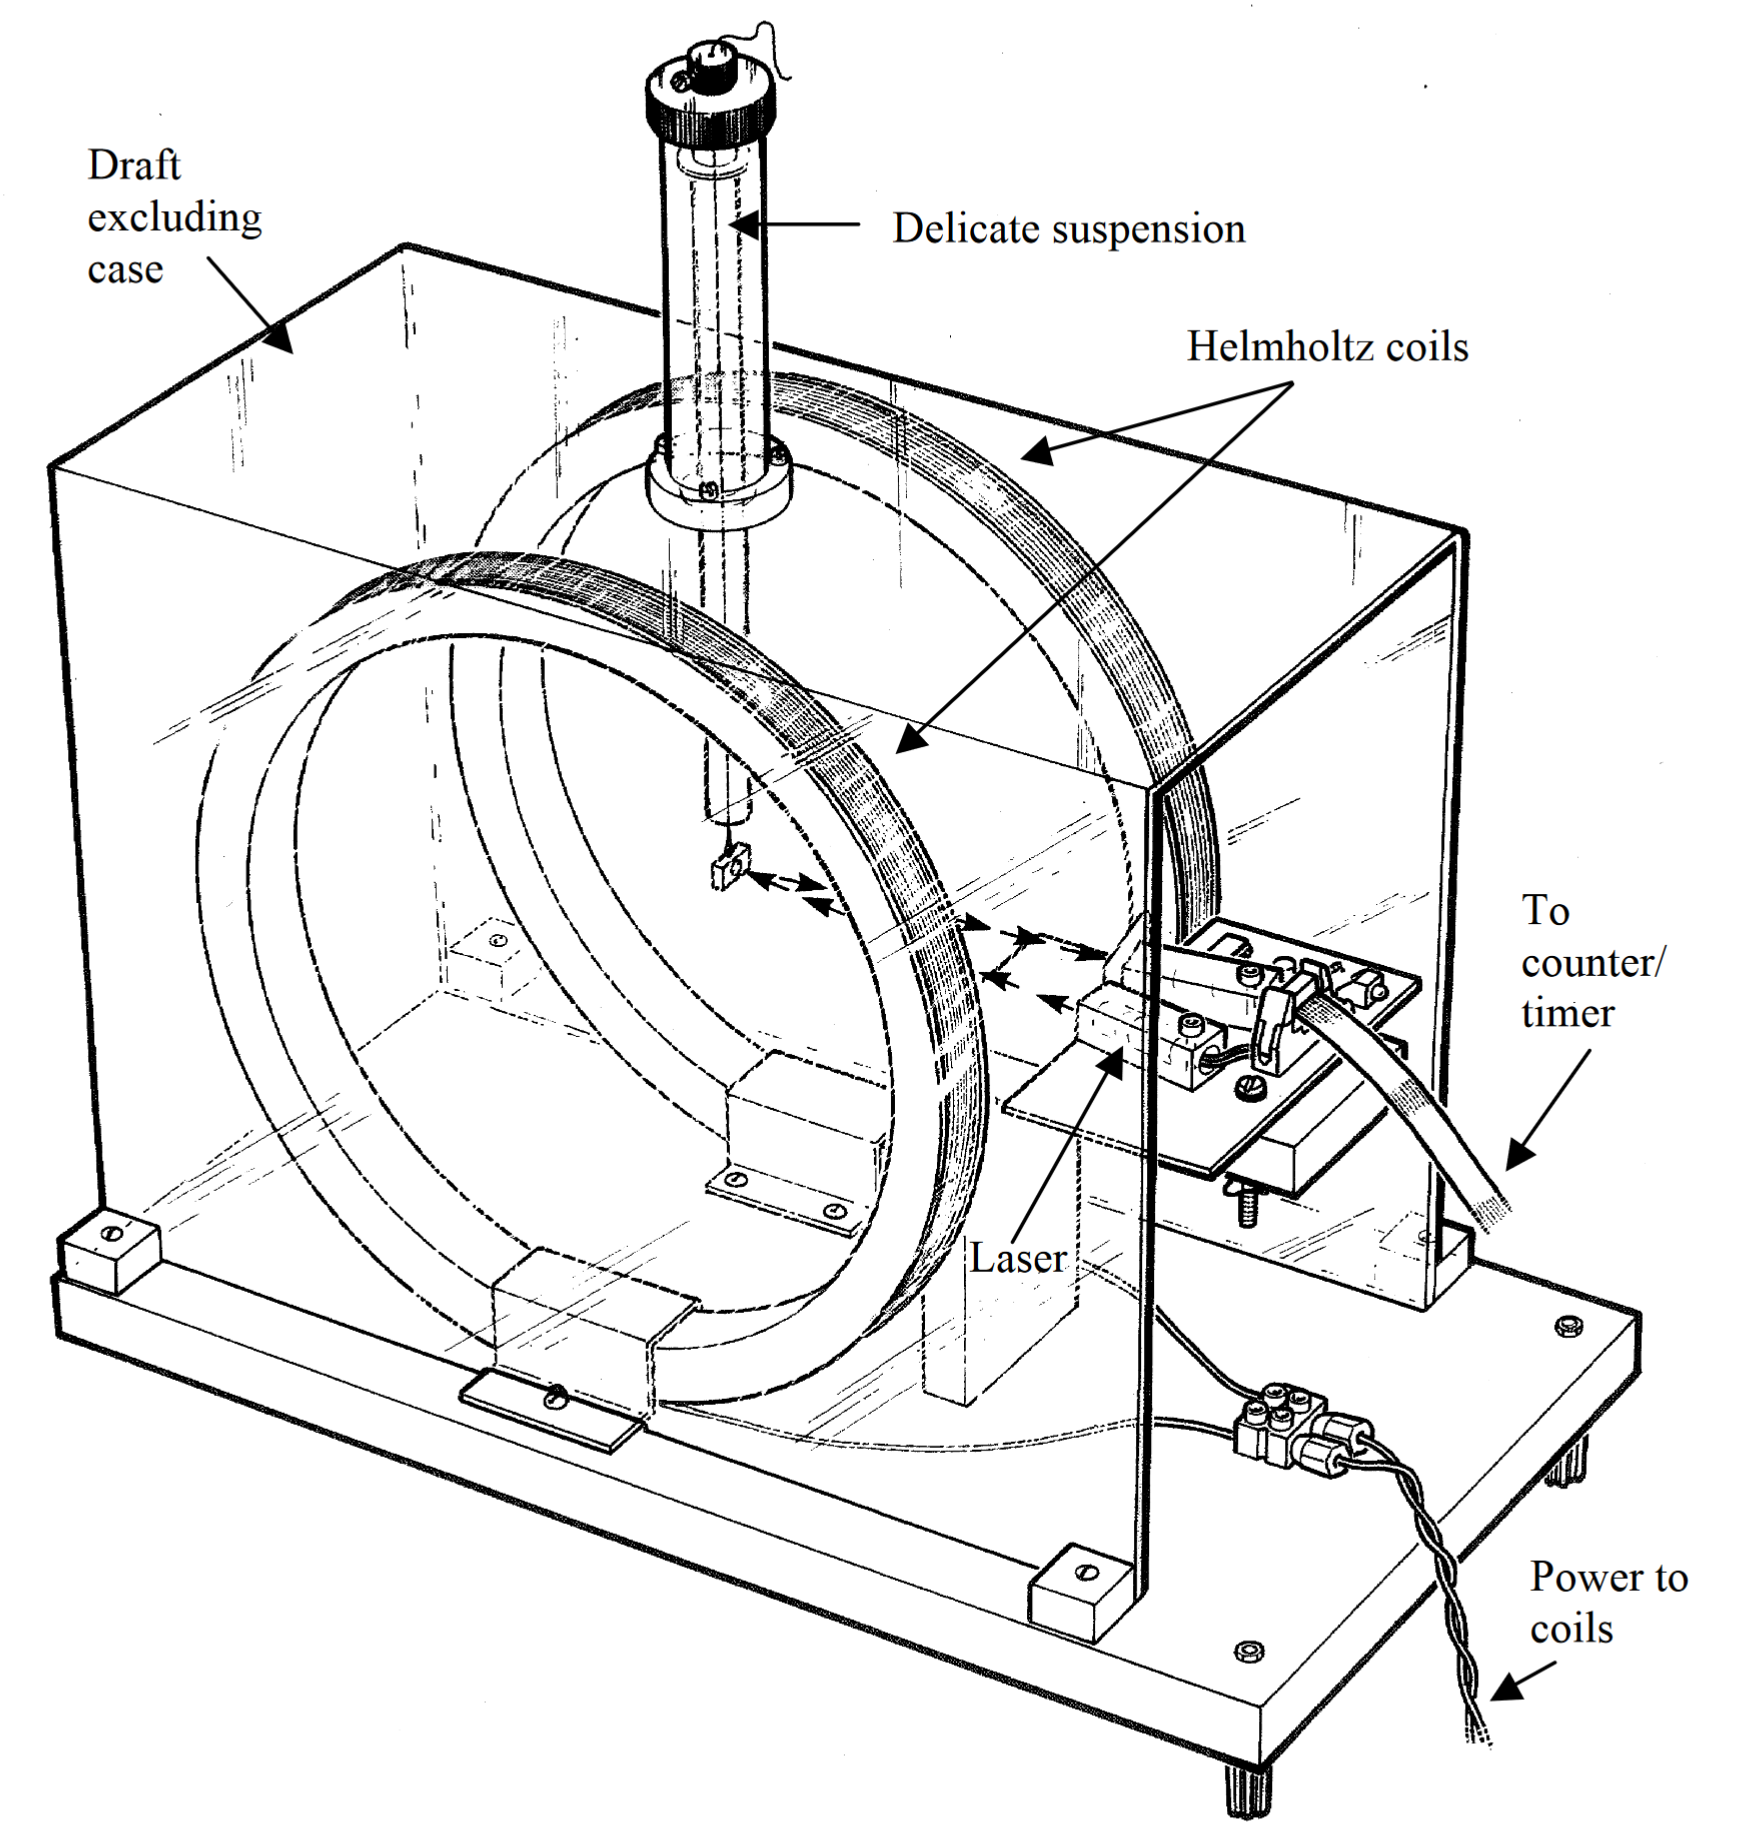
\includegraphics[width=16cm]{images/experimental-setup.png}
  \caption{The experiment\cite{unknown}}
  \label{fig:figure1}
  \end{figure}

To allow the counting device to measure the oscillations it has a little mirror glued onto it. A laser shines onto this
mirror. Depending on the angle of the magnet the laser light will be reflected at a different angle. The light activated
gate is placed such that the light from the laser hits it once per oscillation. \\

The Helmholz coil is connected to a variable power supply. This makes it possible to adjust its field strength to a
a desired known value.


\section{Theory}

We can start by looking at
the magnetic force: 
$$
\tau = \mu \times B
$$

Instead of using the cross product, the formula can be rearranged to be defined as the angle between the magnetic dipole moment
$\mu$ and the magnetic field $B$: 

$$
\tau = -\mu B \sin(\theta)
$$

The negative sign appears as it is a restoring force, such that the magnetic dipole experiences a force aligning it
with the magnetic field.\\

This can be combined with the required torque needed to accelerate an object with inertia $I$:

$$
\tau = I\omega
$$
or
$$
\tau = I\frac{d^2\theta}{dt^2}
$$

thus resulting in (using the small angle approximation $\sin(\theta)=\theta$):

$$
\frac{d^2\theta}{dt^2} + \frac{\mu B \theta}{I} = 0
$$

Solving the differential equation results in:

$$
\omega(t) = e^{\sqrt{-\frac{\mu B}{I}} t}
$$

taking $i$ outside gives us

$$
\omega(t) = e^{i t \sqrt{\frac{\mu B}{I}} }
$$

From this we can get the period $T$:

$$
T = 2 \pi \sqrt{\frac{I}{\mu B}}
$$

\subsection{Moment of inertia}

The moment of inertia for the magnet can be determined by using the definition for the inertia and then
integrating over it:

$$
I = d^2 m
$$

As the magnet is free to spin around the central vertical axis, we need to take the distance to the center:

$$
dd = \sqrt{\frac{1}{2} dl^2 + \frac{1}{2} dw^2}
$$

$$
I = \int_0^l{\int_0^w{(\sqrt{\frac{1}{2} dl^2 + \frac{1}{2} dw^2})^2}}dw dl m
$$

reducing to

\begin{equation}\label{eq_I}
I = \frac{1}{12}(l^2 + w^2) m
\end{equation}

\subsection{Magnetic field}

As the magnetic field of the earth ($B_h$) and Helmholz coils ($B_c$) line up the fields add up, thus:
$$
B = B_h + B_c
$$

with

\begin{equation}\label{eq_bc}
B_c = k i
\end{equation}

and 

\begin{equation}\label{eq_k}
k = \frac{8}{5^{3/2}} \frac{\mu_0 n}{r}
\end{equation}

results In

$$
B = B_h + k i
$$

\subsection{Putting everything together}


$$
T^2 = 2 \pi {\frac{I}{\mu B_{h} + k i}}
$$

$$
1/T^2 = 4 \pi^2 {\frac{\mu B_h + k i}{I}}
$$

\begin{equation}\label{eq_mbx}
1/T^2 = \frac{\mu k}{4 \pi^2 I}i + \frac{\mu B_h}{4 \pi^2 I}
\end{equation}

this now being in the form $y = mx + b$ the slope ($S$) and the intercept ($b$) can be calculated to get the values
for $\mu$ and $B_h$ respectively:

\begin{equation}\label{eq_mu}
 \mu = \frac{S 4 \pi^2 I }{k}
\end{equation}
\\
\begin{equation}\label{eq_bh}
B_h = \frac{4 \pi^2 I b }{\mu }
\end{equation}

\section{Experimental Procedure}
\subsection{Preperation}
The first thing that needs
to be done is align the Helmholtz magnetic field with the magnetic field of the earth. This can be done by utilizing a
compass and aligning the Helmholtz coils in the direction it's pointing. In the case of this experiment the bar
magnet already suspended in the middle of the Helmholz coil's frame can be used as the compass. One just has to
wait until it stops oscillating. After that the coils can then be aligned in the direction the bar magnet is pointing.\\
The Helmholz coils are now aligned in such a way that they could either produce a magnetic field exactly in the direction
of earth magnetic field or exactly opposite to it. To figure out which is the case the coil can be turned on a high setting
(producing a magnetic field bigger than earth's). If the magnet flips violently, the magnetic fields are pointing in the
opposite direction. If not the fields are aligned. Should the magnet flip around, there are three ways to solve this:
\begin{enumerate}
  \item Flip the Helmholz coils around
  \item Flip the polarity of the coils
  \item Add a minus sign to the field strength in equation \ref{eq_mbx}
\end{enumerate}

In our case we simply flipped the polarity as this just required switching around the cables coming from the power
supply.\\

Next the counting device needs to be prepared for measuring the frequency of the oscillation.
The counting device used in the experiment has a setting allowing to measure the time until $n$ number of events
are counted. From this the frequency can be determined as such: $f = n/t$. We chose to set $n$ to 50 to get a
precise measurement.\\

As the last step before recording the measurements, the laser gate has to be set up to be triggered once per oscillation.
To do so the power supply was set to a medium setting. The bar magnet should start oscillating as a result. If not 
it can be manually given a push. The laser can now be turned on. It now needs to be ensured that its beam hits the 
light gate for every oscillation of the magnet. There are two ways to do this:
\begin{enumerate}
  \item Adjust the rotation of the laser, such that it hits the mirror on the magnet at a different angle
  \item Adjust the feet of the frame, such that the magnet (which is suspended from a thread) is being translated
  relative to the laser light gate setup.
\end{enumerate}

The LED on the light gate lights should now light up reliably.

\subsection{Taking the measurements}

With the setup done the measurements can now be taken. To do this the power supply is first set to the desired current.
It is crucial to wait for the current to stabilize before proceeding. This might take a short while as adjusting current
results in the magnetic field changing which in reverse again induces a current.\\
With a stable magnetic field, the counter can now be stared. After the counter is done counting the time should be recorded
and the procedure can be repeated with a new current setting. \\
If the counting becomes unreliable during the experiment (which it did in our case), it might help to give the magnet a
bigger push at the beginning (increasing he oscillation magnitude\footnote{Be careful to not exceed $>5\deg$ to not exceed
the limit of the small-angle approximation used in the formulas}) or by repeating the adjustment step. If this happens
all measurements should get retaken to reduce the error.\\

After taking all the measurements the dimensions and the mass of the magnet needs to be measured and recorded.
This is best done with calipers and a high-precision scale.\\

Furthermore, the constant $k$ for the Helmholtz coil (introduced in equation\ref{eq_k}) needs to be taken or
calculated from the manufacturer's datasheet.

\section{Experimental Results}

We decided to take 10 measurements between $2A$ and $0.2$:\\

\begin{table}[H]
\centering
\label{date_raw}
\begin{tabular}{rrrr}
\toprule
 current &  time &  Frequency &  Frequency\textasciicircum 2 \\
\midrule
     2.0 &  8.03 &     0.1606 &    38.771171 \\
     1.8 &  8.44 &     0.1688 &    35.095797 \\
     1.6 &  8.96 &     0.1792 &    31.140386 \\
     1.4 &  9.47 &     0.1894 &    27.876616 \\
     1.2 & 10.23 &     0.2046 &    23.888492 \\
     1.0 & 11.24 &     0.2248 &    19.788250 \\
     0.8 & 12.66 &     0.2532 &    15.598132 \\
     0.6 & 14.34 &     0.2868 &    12.157428 \\
     0.4 & 17.08 &     0.3416 &     8.569674 \\
     0.2 & 25.56 &     0.5112 &     3.826646 \\
\bottomrule
\end{tabular}
\end{table}


\begin{figure}[H]
  \begin{center}
% This file was created with tikzplotlib v0.10.1.
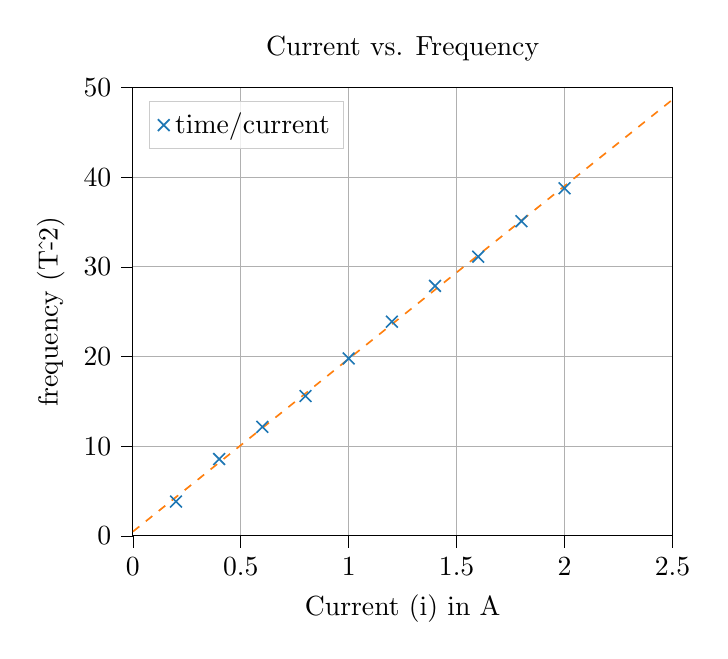
\begin{tikzpicture}

\definecolor{darkgray176}{RGB}{176,176,176}
\definecolor{darkorange25512714}{RGB}{255,127,14}
\definecolor{lightgray204}{RGB}{204,204,204}
\definecolor{steelblue31119180}{RGB}{31,119,180}

\begin{axis}[
legend cell align={left},
legend style={
  fill opacity=0.8,
  draw opacity=1,
  text opacity=1,
  at={(0.03,0.97)},
  anchor=north west,
  draw=lightgray204
},
tick align=outside,
tick pos=left,
title={Current vs. Frequency},
x grid style={darkgray176},
xlabel={Current (i) in A},
xmajorgrids,
xmin=0, xmax=2.5,
xtick style={color=black},
y grid style={darkgray176},
ylabel={frequency (T\^-2)},
ymajorgrids,
ymin=0, ymax=50,
ytick style={color=black}
]
\addplot [semithick, steelblue31119180, mark=x, mark size=3, mark options={solid}, only marks]
table {%
2 38.7711709979234
1.8 35.0957974888255
1.6 31.1403858418367
1.4 27.8766158680388
1.2 23.888492339916
1 19.788249895518
0.8 15.5981322172558
0.6 12.1574279939855
0.4 8.5696735022953
0.2 3.82664619257888
};
\addlegendentry{time/current}
\addplot [semithick, darkorange25512714, dashed, forget plot]
table {%
0 0.470123440823551
2.5 48.654522970355
};
\end{axis}

\end{tikzpicture}

  \end{center}
\end{figure}

We also measured the width, length and mass of the magnet as well as recorded the $k$ value for the Helmholtz
coils used:\\

\begin{table}[H]
\centering
\label{further_consts}
\begin{tabular}{rrrr}
\toprule
 Helmholz coil constant &  Magnet length (l) &  Magnet width (w) &  Magnet mass (m) \\
\midrule
               0.000745 &           0.019897 &          0.005257 &         0.007413 \\
\bottomrule
\end{tabular}
\end{table}



\section{Analysis}

All analysis was done in python. If you need the source code please have a look at the 
\href{https://github.com/sidney-pauly/papers}{github repository}.\\

Analyzing the data is now fairly straightforward. The slope and intercept can be either
read of the graph or as done here be calculated with a regression algorithm:\\

\begin{table}[H]
\centering
\label{slope}
\begin{tabular}{rrrr}
\toprule
   Slope &  Intercept &  Standard deviation &  Standard deviation(\%) \\
\midrule
19.27376 &   0.470123 &            0.293034 &               1.520378 \\
\bottomrule
\end{tabular}
\end{table}


To now calculate the magnetic dipole moment $\mu$ and the strength of earth's magnetic
field $B_h$ we now need the values using formulas \ref{eq_mu} and \ref{eq_bh} respectively, we need
the inertia of the magnet $I$ and the constant $k$ relating the Helmholtz coil's field strength $B_c$ to current.\\
$k$ can be found in table\ref{further_consts}. The inertia was calculated from the values in the same table
using formula\ref{eq_I}. Plugging everything into formulas \ref{eq_mu} and \ref{eq_bh} gives the following
final results:\\

\begin{table}[H]
\centering
\label{end_result}
\begin{tabular}{rrrrr}
\toprule
 Intertia (I) &  Dipole Moment &  Earth magnetic field (expected) &  Earth magnetic field (measured) &    Error \\
\midrule
 2.616384e-07 &        0.33928 &                         0.000017 &                         0.000018 & 1.101331 \\
\bottomrule
\end{tabular}
\end{table}


\section{Discussion}

The final calculated result is just 10\% off from the expected value. While the result agrees with the literature
value it is not really precise. From the linear regression \ref{slope} we can see that the standard division
of the measurements is only around 1.5\% which does not explain the final error of >10\%. This means the error
either comes from one of the other measurements taken (Magnetic field strength or dimensions/weight of the magnet)
or it's a systematic error.\\

While the error could very well come from the other measurements, it's more likely that it is a systematic error.\\

There are four possible identifiable causes for such a systematic error:

\begin{enumerate}
\item Small-angle approximation: the small-angle approximation is just that: an approximation so this might contribute to the error
\item The two magnetic fields might not be aligned perfectly, therefore their forces would not exactly add up
\item The thread on which the magnet is suspended could introduce a torque, thus, the magnetic torque would
      not be the only relevant force
\item Foreign objects could interfere with the magnetic field around the experiment. In the setting of the experiment
      this is quite likely as there were multiple experiments utilizing magnetic fields running in the same lab at the same time
\end{enumerate}

\printbibliography

\end{document}
